% ! TeX root = ../document.tex
\begin{frame}<6>{Collective Adapative Systems: Challenges}
  %% Background
  \only<1-4>{ 
    \begin{backgroundblock} 
      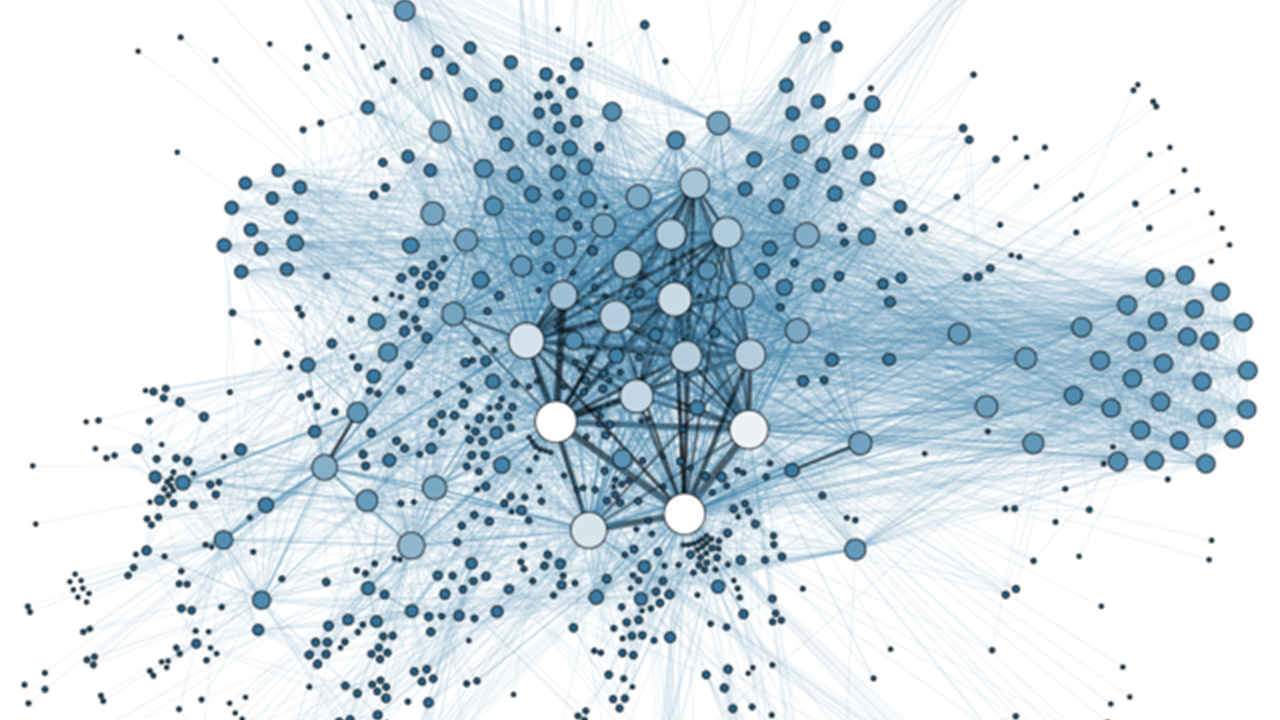
\includegraphics[width=\paperwidth]{img/complex-network.png} 
    \end{backgroundblock} 
  }
  \only<5-6>{ 
    \begin{backgroundblock} 
      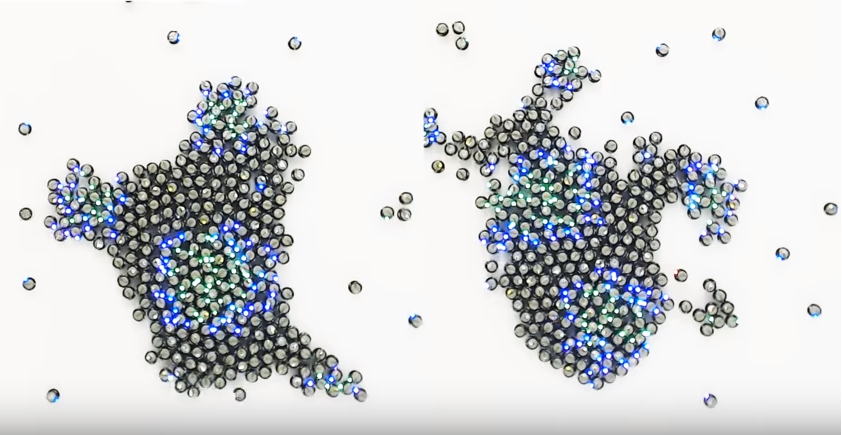
\includegraphics[height=\paperheight]{img/swarms.png}
    \end{backgroundblock} 
  }
  \begin{card}
    \begin{itemize}
      \item<1-> Complex and layered networks
      \begin{itemize}
        \item <2->Large scale
        \item <3->Heterogenous
        \item <4->Dynamic
      \end{itemize}
      \item<5-> Distributed control
      \item<6-> Environmental changes
    \end{itemize}
  \end{card}

  \begin{cardRed}[Engineering problem]
    \begin{itemize}
      \item Is it possible to define a collective behaviour indipedently from the network topology?
    \end{itemize}
  \end{cardRed}
\end{frame}